\section{Results}
\label{sec:results}

Section~\ref{sec:devres} summarises the development results that set the hypotheses; they are numerical and were produced on 2023 data. Sections~\ref{sec:confres} to~\ref{sec:h8} report the single confirmatory run on the 31 sealed sites. Pairs of values are independent loss and Gilbert loss, with loss probability 0.3 and $Q = 6$ unless stated.

\subsection{Development results}
\label{sec:devres}
On the 38 development sites (10,342 four-parameter days), the findings that shaped the pre-registration were the following:
\begin{itemize}
  \item Soundness: no certificate design gave a wrong decision in any condition.
  \item Witnesses added decisions: the record alone decided 0.677 of hard cases at the configured thresholds (independent loss), and the 3b rule 0.968. A witness placed inside the record code did almost nothing for the 7DADM, which needs seven informative days; placement in a protected group mattered.
  \item Targeting paid: against the same layering on random days, the 3b rule gained 0.10 to 0.15 on near 7DADM windows and 0.17 on hard conductance days, at a record-recovery cost of 0.001 to 0.005.
  \item The exact allocator did not beat the simple rule on hard cases, and the pre-registered criterion for it was not met; the simple rule was within 7\% (at $Q = 6$) and 1.6\% (at $Q = 12$) of the optimum of the stated objective.
  \item Decision flags dominated on thresholds known at configuration time: flags decided 0.999 of hard cases against 0.968 for the 3b rule, and recovered the record more often. On two threshold sets that the encoder did not know, the 3b rule exceeded the flags by 0.42 to 0.57.
  \item Send-on-delta needed 1.79 times as many values as the piecewise-linear record, and a tightened tolerance did not improve hard-case decisions at this quota.
  \item Hybrid 1 matched the flags on configured thresholds and record recovery and gained 0.416 and 0.355 on the unanticipated thresholds; hybrid 2 lost record recovery. Hybrid 1 therefore met the adoption rule that was written in advance and was adopted before the freeze.
\end{itemize}

\subsection{Confirmation: nine hypotheses}
\label{sec:confres}
Table~\ref{tab:hyp} lists every hypothesis with its limit, its result, and its outcome; eight were supported and H8 was not. The run completed without interruption: the freeze check passed, 31 of 31 checksums verified, and the log contains no error.
\begin{itemize}
  \item H1, soundness: the maximum share of wrong certain decisions was 0.000 in every certificate design at $Q = 6$ and $Q = 12$ under both loss models, and the byte-level round trip of frame version 2 showed no mismatch in 30,285 blocks. The caveat of Section~\ref{sec:procedure} applies.
  \item H2, benefit over the record alone: the 3b rule decided 0.318 (0.234 to 0.417) more hard cases at the configured thresholds under independent loss and 0.300 (0.223 to 0.390) under bursts, against a limit of 0.15.
  \item H3, value of targeting: against the same layering on random days, the gain was 0.141 (0.105 to 0.174) and 0.130 (0.096 to 0.165), against a limit of 0.05.
  \item H4, cost in record recovery: the 3b rule recovered the record less often than the record alone, by 0.083 (0.062 to 0.105) and 0.071 (0.053 to 0.091). The pre-registered limit was 0.12, and this was the hypothesis with the thinnest margin in development; it held, and the lower bound of the loss was 0.105 under independent loss.
  \item H5, generality: on thresholds that the encoder did not know, the 3b rule exceeded the flags by 0.531 (0.494 to 0.569) and 0.441 (0.411 to 0.472), and the record alone by 0.260 (0.191 to 0.344) and 0.245 (0.184 to 0.320).
  \item H6, baselines: neither coded send-on-delta nor a tolerance multiplied by 0.5 dominated the 3b rule in any of the four combinations.
  \item H7, the known limit: the flags exceeded the 3b rule in hard-case decisions at the configured thresholds by 0.043 (0.025 to 0.068) under independent loss. This replicated the development finding and is a limit of the witness design, not a success.
  \item H9, the hybrid: hybrid 1 exceeded the flags on the unanticipated thresholds by 0.355 (0.297 to 0.418) and 0.294 (0.248 to 0.345), and matched them exactly on configured hard-case decisions and on record recovery (0.000 in all four contrasts).
\end{itemize}

Fig.~\ref{fig:forest} shows the contrasts with their intervals and limits.

\begin{figure}[t]
\centering
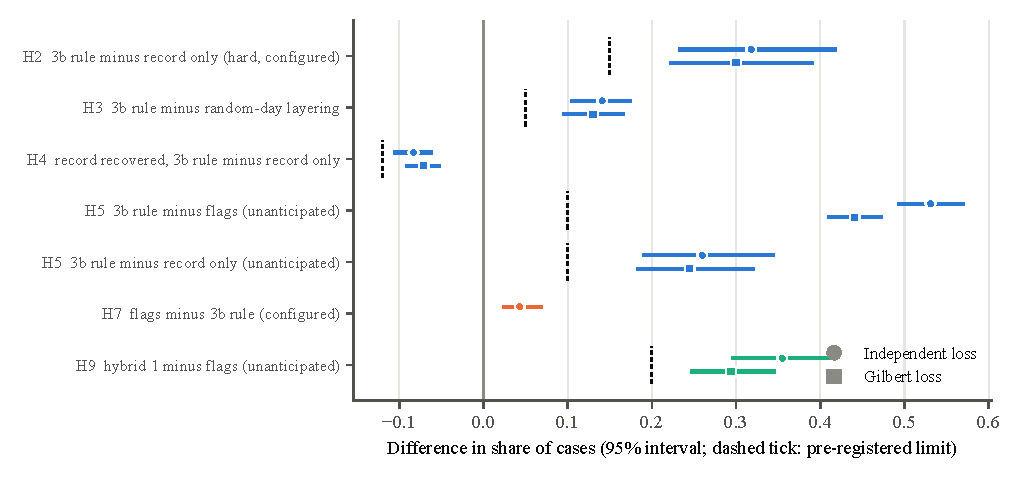
\includegraphics[width=\textwidth]{figs/forest.pdf}
\caption{Confirmed contrasts at six messages per day with 95\% site-clustered intervals; the dashed tick marks the pre-registered limit of each hypothesis. Circles are independent loss and squares are Gilbert loss. Blue marks contrasts of the 3b rule, orange the known limit (H7), and green the hybrid (H9).}
\label{fig:forest}
\end{figure}

\subsection{Descriptive comparison of all designs}
\label{sec:desc}
Table~\ref{tab:desc} and Fig.~\ref{fig:tradeoff} show the pooled levels of every design at $Q = 6$; these results carry no verdict.
\begin{itemize}
  \item The flags decided 0.999 of hard cases at configured thresholds under independent loss but only 0.275 on unanticipated thresholds; hybrid 1 kept the flag performance and raised the unanticipated level to 0.629 without reducing record recovery (0.877 for both).
  \item Hybrid 2 reached 0.806 on unanticipated thresholds, the same as the 3b rule, but recovered the record less often (0.779 against 0.877 for the flags).
  \item The exact allocator, relative to the 3b rule, changed record recovery by +0.028, hard configured decisions by $-$0.015, hard unanticipated decisions by $-$0.057, and all configured decisions by +0.049 under independent loss. As in development, it did not beat the simple rule on hard cases; therefore, no confirmatory claim is made for it.
  \item Send-on-delta and the tightened tolerance were below the record alone in record recovery and in hard-case decisions at this quota.
  \item At $Q = 12$ the orderings were the same at higher levels: for example, under independent loss the record alone recovered the record in 0.972 of days and the flags and hybrid 1 in 0.969. The full tables are in the supplementary results file of the confirmation.
\end{itemize}


\begin{figure}[t]
\centering
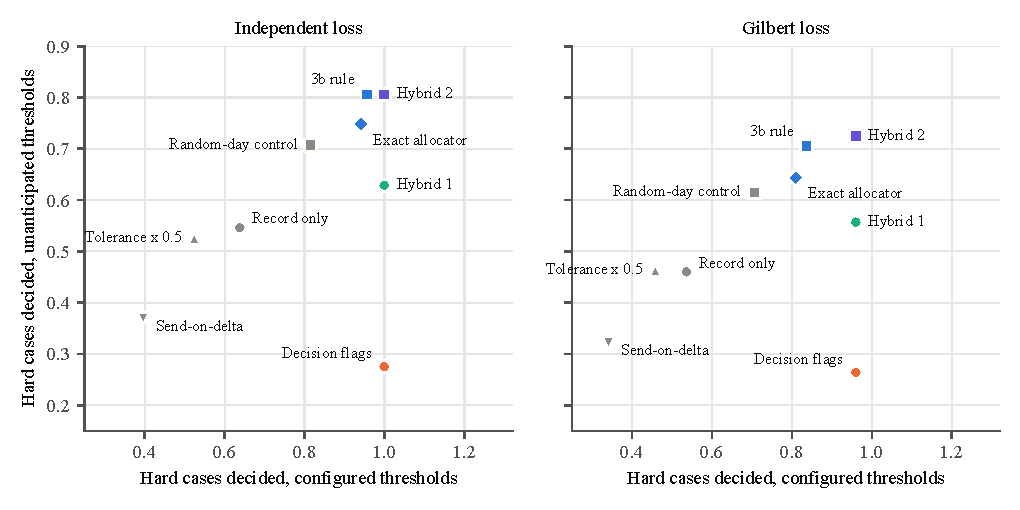
\includegraphics[width=\textwidth]{figs/tradeoff.pdf}
\caption{Trade-off between decisions at configured and unanticipated thresholds for every design at six messages per day (pooled hard cases). Flags decide almost every configured hard case but few unanticipated ones; hybrid 1 keeps the flag level on configured thresholds and raises the unanticipated level; the layered designs reach the highest unanticipated level.}
\label{fig:tradeoff}
\end{figure}

\begin{table}[!htbp]
\centering
\caption{Pooled levels of every design at six messages per day (record recovered, hard cases at configured thresholds, hard cases at unanticipated thresholds, and all days at configured thresholds).}
\label{tab:desc}
\small
\begin{tabular}{@{}lrrrr@{}}
\toprule
Design & Record & Hard, configured & Hard, unanticipated & All, configured \\
\midrule
\tableinput{tables/confirm_desc.tex}
\bottomrule
\end{tabular}
\end{table}

\subsection{Integrity under a forged message: H8 failed}
\label{sec:h8}
H8 bounded the share of days with a false certificate after one message that passes the CRC-16 and replaces an arrived message, given the full receiver (CRC, sanity, and corroboration). Two of its four bounds were exceeded; therefore, the hypothesis was not supported:
\begin{itemize}
  \item Record only, $Q = 6$: 0.0463, with an upper bound of 0.0584 against a limit of 0.06. Within the limit.
  \item Record only, $Q = 12$: 0.0061, with an upper bound of 0.0134 against a limit of 0.01. Exceeded; the point estimate lay inside the limit and the upper bound did not.
  \item Layered witnesses with $k_w = 2$, $Q = 6$: 0.1050, with an upper bound of 0.1197 against a limit of 0.15. Within the limit.
  \item Layered witnesses with $k_w = 2$, $Q = 12$: 0.0126, with an upper bound of 0.0215 against a limit of 0.02. Exceeded, in the same way.
\end{itemize}
Fig.~\ref{fig:h8} compares the cohort with the development estimates and the limits.

\begin{figure}[t]
\centering
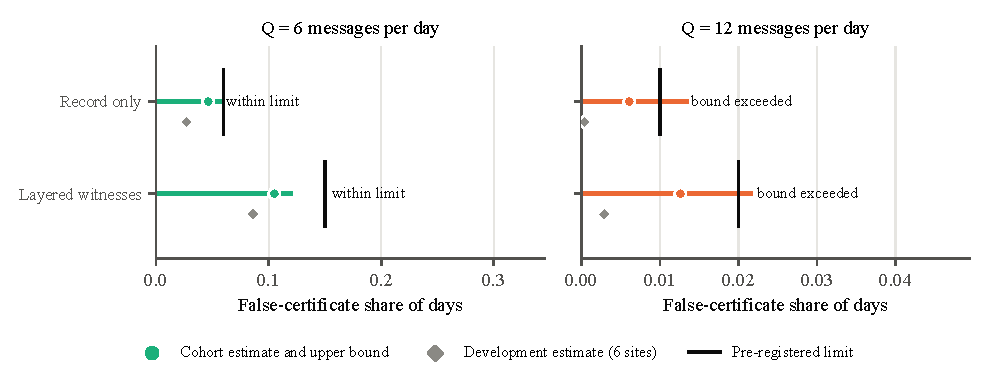
\includegraphics[width=0.9\textwidth]{figs/h8.pdf}
\caption{Share of days with a false certificate after one CRC-valid forgery, with the full receiver. Dots are cohort estimates with their upper bounds; diamonds are the development estimates from six sites; the vertical line is the pre-registered limit. The bounds at twelve messages per day exceeded their limits.}
\label{fig:h8}
\end{figure}

Every cohort value was higher than the corresponding development value from six sites (0.027, 0.0004, 0.086, and 0.0029); the record-only value at $Q = 12$ was about 15 times higher. The development estimate was therefore optimistic. The forgeries are random-content forgeries conditional on a CRC pass, and the absolute rate of false certificates also depends on the real error rate of the channel, which is unknown. The unconditional rate, under a model with a 16-bit pass probability, was not tested in the confirmation. A longer check is the obvious remedy: in development, a CRC-24 cut the forgery rate 256-fold by the capacity argument and reduced fully recovered records from 0.915 to 0.862 at $Q = 6$; its effect on the cohort was not tested and no limit was changed.
